\chapter{Предметная область} \label{chapt1}
% % %todo убрать висящие строки
Данные о плотности грунта служат основанием для оценки залежей полезных ископаемых 
и принятия решения о начале геологоразведки перспективных районов. На основании  информации о плотности грунта 
определяются порядок, объем и состав проектных работ при подготовке к строительству зданий и дорог, делаются заключения о безопасности проводимых 
строительных работ, качестве их выполнения и возможности ввода в эксплуатацию возведенных сооружений. При подготовке ряда объектов 
(фундаментов зданий, шоссе, железнодорожных насыпей) проводятся работы по уплотнению грунта,
 для определения объема которых необходимы измеренные и требуемые значения показателей плотности сухого грунта.
Мониторинг плотности грунта позволяет контролировать и упреждать возникновение аварийных ситуаций при эксплуатации возведенных объектов, 
в частности, таких, как высотные здания, мосты, железнодорожные насыпи, линии метро, шахты, аэродромы.

\section[Методы измерения плотности грунта в геологии]{ Методы измерения плотности грунта \\ в~геологии} \label{sect1_1}

Плотность грунта измеряется контактными методами через непосредственный замер плотности образцов, 
или бесконтактными (радиационными методами). 
В обоих случаях предполагается бурение исследуемого грунта. 

\subsection{Контактные методы}\label{subsect1_1_1}

В ГОСТ-5180-84. ``Грунты. Методы лабораторного определения физических характеристик`` \cite{gost5180} описаны следующие 
методы измерения плотности грунта: режущим кольцом, взвешивание в воде парафинированных образцов, и 
взвешивание мерзлых пород в нейтральных жидкостях. В зависимости от типа грунта, его сыпучести и содержания воды,
выбирается тот или иной метод. Масса образца грунта составляет от двухсот грамм до нескольких килограммов. При этом, чтобы получить 
распределение плотности грунта, проводится ряд параллельных замеров. Значение характеристик вычисляют, как 
среднее арифметическое из результатов параллельных измерений. 
Разница между параллельными измерениями не должна превышать значений, указанных в приложении к ГОСТ-5180-84. 
Если разница превышает допустимую, количество измерений следует увеличить.

Главный недостаток контактных методов --- локальный характер измерения плотности грунта, связанные с этим проблемы с определением 
неоднородностей (полости, каверны) в грунте. Во время эксплуатации объектов подобные неоднородности могут привести к обрушениям или осадке фундамента. 
Цена за низкую погрешность итоговых значений плотности --- чрезмерный объем бурильных и лабораторных работ. 

%\textit{По ссылке --- статья про женщину, под которой провалился асфальт от того, что грунт вымыло потоком воды, я не знаю включать ли этот случай в текст 
%диплома} 
%
%http://www.bbc.co.uk/russian/russia/2012/01/120108\_bryansk\_toddler\_killed.shtml

\subsection{Бесконтактные методы}\label{subsect1_1_2}

Метод радиоизотопного измерения плотности грунтов основан на зависимости между плотностью контролируемого 
грунта и характеристиками ослабления и рассеяния измеряемого потока энергии гамма-излучения.

Плотность грунта измеряется путем детектирования и регистрации плотности потока рассеянного первичного 
гамма-излучения (метод альбедо), ослабленного первичного гамма-излучения (метод абсорбции) или 
рассеянного и ослабленного первичного гамма-излучения (альбедно-абсорбционный метод).

Метод альбедо заключается в регистрации плотности потока гамма-квантов, рассеянных на электронах атомов 
вещества при взаимодействии потока энергии первичного гамма-излучения источника ионизирующего излучения с материалом грунта.
Метод абсорбции --- в детектировании плотности потока гамма-квантов, прошедших через слой материала 
между радиоактивным источником и детектором гамма-излучения.
Альбедо-абсорбционный метод заключается в определении плотности потока гамма-квантов, рассеянных 
в объеме грунта и прошедших через слой между источником ионизирующего излучения и детектором гамма-излучения.

При проведении измерений радиоизотопными плотномерами, должны соблюдаться ``Основные санитарные правила работы с 
радиоактивными веществами и другими источниками ионизирующих излучений``, ``Нормы радиационной безопасности``, 
``Правила безопасности при транспортировании радиоактивных веществ``.

Радиационный метод обеспечивает комплексную оценку исследуемого объекта, однако не лишен недостатков --- используются
радиоактивные вещества, представляющие опасность для здоровья.


Эти обстоятельства стимулируют исследователей искать альтернативные подходы к измерению плотности грунта. 
Один из недавно предложенных способов, исследуемый в Институте автоматики и электрометрии СО РАН \cite{patentdensitometer} ---
использование в качестве источника радиации естественный радиационный фон --- атмосферные мюоны. 
Обладая достоинствами радиационных методов, мюонный плотномер 
не использует активных источников радиации и, соответственно, безопасен для здоровья. 

\section[Физическая модель рождения мюонов]{Физическая модель рождения мюонов \\ и их поглощения в веществе}\label{sect1_2}

Источником атмосферных мюонов является взаимодействие высокоэнергетичных космических частиц (Первичные Космические Лучи) с верхними слоями атмосферы. В модели В. И. Зацепина \cite{zacepin}. предполагается существование трех классов источников космических лучей --- взрывов сверхновых и новых разного типа :
\begin{enumerate}
	\item I класс --- ударные волны от массивных взрывающихся скоплений (ассоциаций) сверхновых спектрального класса О или В;
	\item II класс --- ударные волны от неассоциированных сверхновых звезд, взрывающихся в случайную межзвездную среду;
	\item III класс --- определяется спектром меньшей жесткости, возможными физическими объектами в этом классе могли бы быть взрывы новых звезд.
\end{enumerate}

Основные рассматриваемые данной моделью группы ядер --- протоны (P), гелий (He), группа  средних ядер -- углерод, азот, кислород (C, N, O), группа тяжелых ядер от неона до серы (Ne--S) и группа очень тяжелых ядер от хлора до никеля (Z > 17). 

Данная модель оспользует следующие положения:

\begin{enumerate}
	\item Ядра космических лучей высоких энергий останавливаются в верхних слоях атмосферы за счет ядро-ядерных столкновений;
	\item При взаимодействии ультрарелятивистской частицы с ядром вторичные частицы вылетают в направлении первичной;
	\item Первичные Космические Лучи имеют равномерное пространственное распределение.
\end{enumerate}

Таким образом, в данном приближении, в верхних 10-15 км атмосферы рождаются потоки вторичных космических частиц, образующих сферические волны, которые приходят на поверхность Земли.

В результате ядро-ядерного взаимодействия происходят следующие превращения частиц:

\begin{equation}
\begin{split}
	\pi &\to \mu + \nu_\mu; \\
	K^\pm &\to \mu^\pm + \nu_\mu (\-{\nu_\mu}); \\
	K^\pm &\to \pi^0 + \mu^\pm + \nu_\mu (\-{\nu_\mu}); \\
	K^0 &\to \pi^\pm + \mu^\mp + \nu_\mu (\-{\nu_\mu}). 
\end{split}
\end{equation}

Кроме того происходят цепочки распадов $K \to \pi \to \mu$.


Атмосферные мюоны --- релятивистские частицы, они имеют энергию от десятков ГэВ до единиц ТэВ и высокую проникающую способность ( характерное ослабление в е раз на 10 м. в. э.). 
В зависимости от энергии эти мюоны могут проникать на глубины 
до нескольких тысяч метров ниже уровня моря и более. Величина 
потока мюонов на различных глубинах определяется 
энергетическим спектром и составом породы, 
а также физикой взаимодействия мюонов с веществом. Но общая 
закономерность --- ее монотонное падение с увеличением глубины. 
Второе значимое обстоятельство, позволяющее использовать мюоны 
в практических целях измерения плотности грунта, --- относительное 
постоянство их интенсивности во времени. Поэтому 
в геологических задачах, когда точность регистрации 
интенсивности не более 3--5 процентов,  
изменениями в интенсивности пренебрегают.

\section{Устройство и работа мюонного плотномера}\label{sect1_3}

\subsection[Принцип измерения плотности породы]{Принцип измерения плотности породы \\ по тарировочной кривой}\label{subsect1_3_1}

В мюонных плотномерах используется абсорбционный метод, 
основанный на замере потока мюонов при прохождении
через вещество. Интенсивность потока мюонов определяется 
средней плотностью горных пород над точкой наблюдения, 
поэтому в качестве единицы измерения глубины 
при наблюдениях в шахтах используют метры водного эквивалента, сокращенно --- \textit{м. в. э.}. 

При измерении в исследуемом грунте делается скважина, 
в скважину опускается прибор, включающий сцинтилляционный датчик, 
и замеряется поток частиц на разных глубинах. 
Тарировочная зависимость интенсивности потока 
мюонов от глубины в м. в. э. позволяет найти глубину 
в м. в. э., соответствующую измеренному потоку мюонов,
а затем по фактическим глубинам, на которых делались замеры, 
определить среднюю плотность вещества между точками измерения:


% % %todo единицы измерения \rho
% % %Рис. 1. Маансарнспр
\begin{equation}
	\label{eq:density}
	\rho = \frac{H_{m.w.e.}(I_1) - H_{m.w.e.}(I_2)}{H_1-H_2}
\end{equation}


$H_{m.w.e.}(I_1)$ --- глубина в м. в. э. для интенсивности потока мюонов $I_1$, измеренной на глубине $H_1$.


$H_{m.w.e.}(I_2)$ --- глубина в м. в. э. для интенсивности потока мюонов $I_2$, измеренной на глубине $H_2$.

Однако известные приборы громоздки и требуют больших затрат времени 
на проведение измерений, что делает их малопригодными для практического 
использования в инженерной геологии и строительстве. 

Для повышения точности измерений необходимо учитывать и свести 
к минимуму статистическую погрешность регистрации скорости 
счета и систематическую погрешность, возникающую при 
изготовлении скважины в зависимости от свойств грунта и 
диаметра скважины.

\subsection{Пилотный вариант мюонного скважинного \\ плотномера}\label{subsect1_3_2}

\begin{figure}[h] 
  \center
  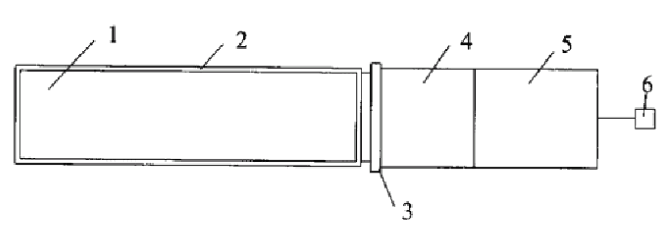
\includegraphics [scale=0.65] {muondensitometer}
  \caption{Датчик мюонного плотномера} 
  \label{img:muondensitometer} 

\end{figure}



В целях снижения временных затрат на измерения с понижением погрешности была предложена конструкция датчика мюонного 
скважинного плотномера (Рис. 1), включающая сцинтилляционный 
детектор (1) с оболочкой (2) и стеклом окна (3), 
фотоумножитель (ФЭУ) (4), усилитель-дискриминатор (5) 
и пульт управления (6).

Физическая длина сцинтилляционного детектора выбирается из 
следующих ограничений. Сцинтилляционная вспышка, 
возникшая на максимальном удалении от фотокатода ФЭУ 
при взаимодействии с мюоном, должна при достижении фотокатода 
иметь достаточно высокий уровень, позволяющий отделить это 
событие от сцинтилляционных вспышек, обусловленных 
естественной радиоактивностью породы, которые 
возникают в непосредственной близости от ФЭУ. Это условие 
ограничивает длину сцинтилляционного детектора сверху и 
зависит от коэффициента ослабления света сцинтилляции, 
который для различных сцинтилляционных материалов может 
быть определен расчетом или экспериментально. 

В усилителе-дискриминаторе предусмотрен регулируемый по 
пространственному разрешению плотности порог дискриминации. 
Это позволяет исключить при измерении вклад естественной 
радиоактивности в зависимости от радионуклидов, содержащихся в 
исследуемом грунте, а также регулировать длину рабочего участка 
сцинтилляционного детектора, тем самым настраивая разрешение под 
требования задачи.

В датчике могут быть использованы неорганические, 
органические, пластические и жидкие сцинтилляционные материалы,
что позволяет варьировать как габариты датчика, 
так и его стоимость. 




Предложенная конструкция мюонного скважинного плотномера  
реализована в пилотном варианте (рис. \ref{img:muondensitometer2}). Плотномер имеет 
герметичный металлический корпус, рассчитанный под диаметр 
обсадной трубы 76 мм. В качестве сцинтилляционного материала 
использован $NaJ(Tl)$. В состав прибора включен 
фотоэлектронный умножитель ФЭУ-93 и  усилитель-дискриминатор, 
выполненный на триггере Шмидта, выход которого согласован с 
блоком управления. Блок управления и регистрации представляет 
собой серийно выпускаемый счетчик импульсов от радиоизотопного 
плотномера ППГР-1. Питание плотномера осуществляется от 
портативного приборного аккумулятора 12 В, 3 А$*$ч. 
Эксплуатационные характеристики макетного варианта 
 опробованы при замере зависимости интенсивности потока 
мюонов от глубины, на воде. 

\begin{figure}[h] 
  \center
  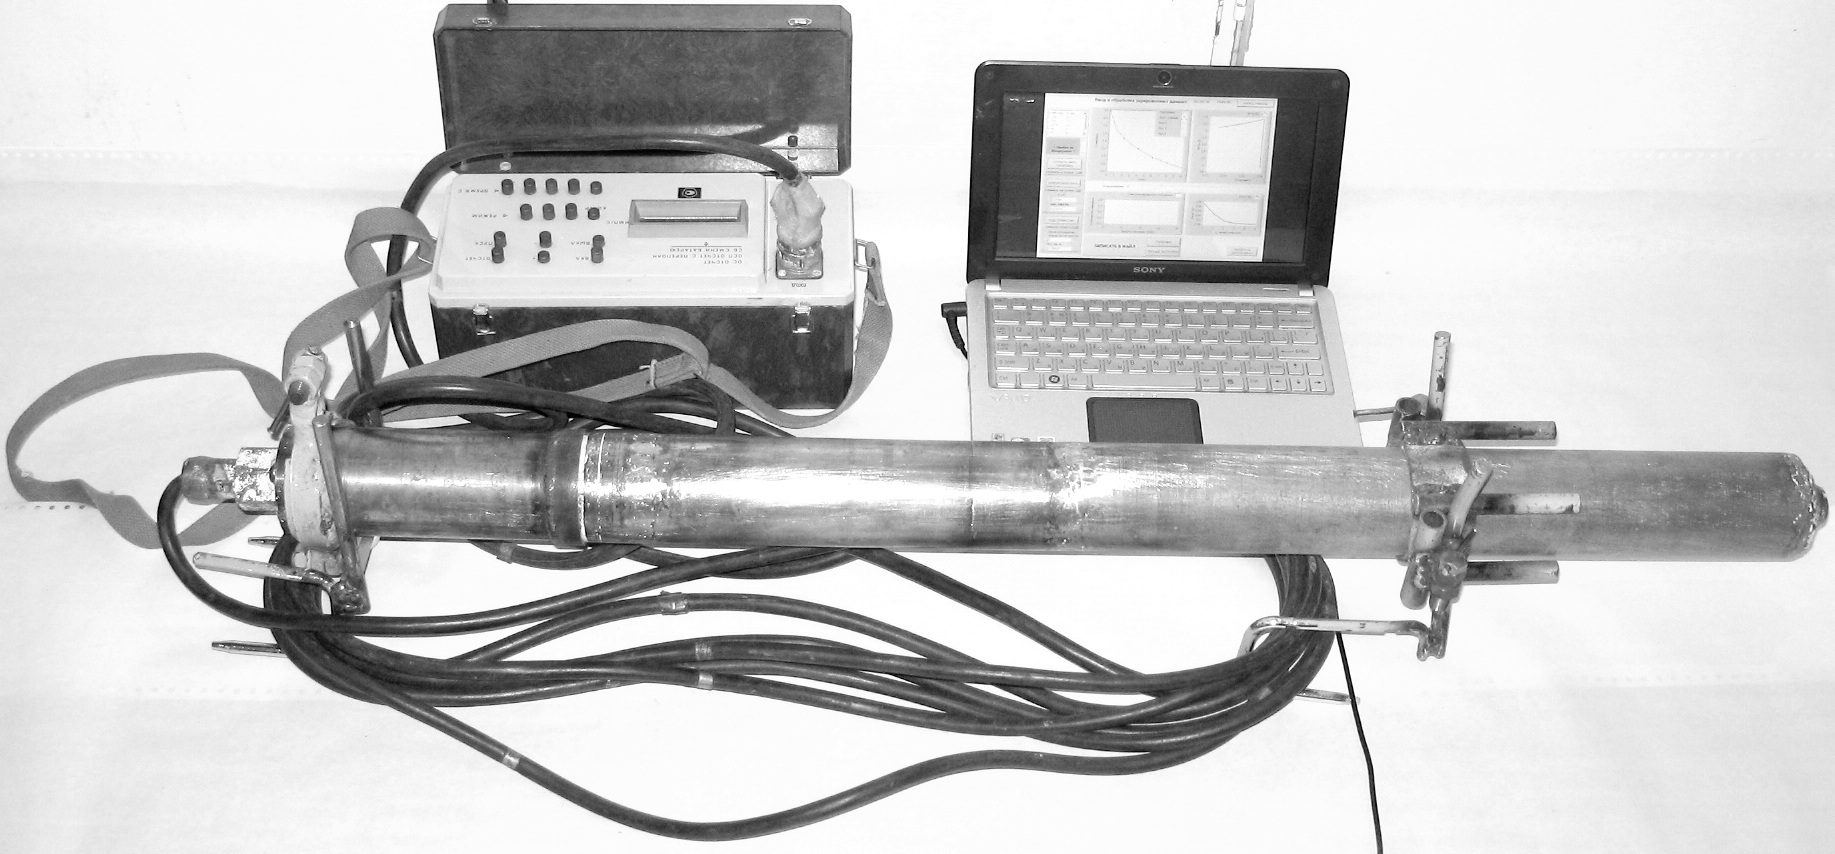
\includegraphics [scale=0.25] {muondensitometer2}
  \caption{Фотография мюонного плотномера} 
  \label{img:muondensitometer2} 

\end{figure}

Резюмируя достоинства переносного скважинного  мюонного плотномера следует отметить:
\begin{itemize}
  \item Экологическую и биологическую безопасность прибора и 
  связанную с этим простоту эксплуатации при хранении, 
  транспортировке. Отсутствие необходимости в 
  согласованиях его использования с санитарно-эпидемиологическими 
  службами.
  \item Простоту калибровки датчика, не требующей специальных 
  приспособлений. Калибровку проводят в открытых естественных 
  водоемах, на воде – жидкости с низким коэффициентом сжатия. 
  \item Существенное снижение (до четырех раз) объема 
  буровых работ  за счет интегрального характера обследования, 
  значимое особенно в случае дисперсионных грунтов.
  \item Практически приемлемую погрешность (порядка 3\%) и 
  продолжительность измерений (не более 60 минут для глубин до 
  20 м. в. э.).
  \item Компактную конструкцию прибора (длина 0.9 м, масса 7 кг) 
  и простоту его эксплуатации в автономном режиме в течение 8 
  часов непрерывной работы.
\end{itemize}

\clearpage